% !TeX program = lualatex
% !TeX encoding = utf8
% !TeX spellcheck = uk_UA
% !TeX root =../MexPractEng.tex

%=========================================================
\chapter{Work and Energy. Laws of Conservations}\label{\currfilebase}
\Opensolutionfile{answer}[\currfilebase/\currfilebase-Answers]
\Writetofile{answer}{\protect\section*{\nameref*{\currfilebase}}}%
%=========================================================

\section{Kinetic Energy and Work}


%%=========================================================
%\begin{problem}
%	A proton (mass $m = 1.67 \cdot 10^{-27}$~kg) is being accelerated
%	along a straight line at $3.6 \cdot 10^{15}$~\si{\meter\per\square\second} in a machine. If the proton
%	has an initial speed of $2.4 \cdot 10^7$~\si{\meter\per\second} and travels $3.5$~cm, what
%	then is 
%	\begin{enumerate*}[label=\alph*)]
%		\item its velocity and
%		\item the increase in its kinetic energy?
%	\end{enumerate*}
%	\begin{solution}
%		\begin{enumerate*}[label=(\alph*)]
%			\item $2.9 \cdot 10^7$~m/s; 
%			\item $2.1 \cdot 10^{13}$~J.
%		\end{enumerate*}
%	\end{solution}
%\end{problem}


%=========================================================
\begin{problem}\label{prb:trunk}
		\addpic{2}{5.5cm}{
		\begin{tikzpicture}
			\pgfmathsetmacro{\fangle}{60}
			\tikzstyle{ground}=[fill,pattern=north east lines,draw=none,minimum width=2cm,minimum height=0.3cm]
			\node (wall1) [ground, minimum width=4cm,yshift=-0.15cm] {};
			\draw (wall1.north west) -- (wall1.north east);
			\fill[red!50, draw=black] (-1,0) rectangle +(2,2) [add reference=BP];
			\draw[-{Latex[open]}, thick, blue] (BP center) -- +(\fangle:3) node[right] {$\vec F_2$};
			\draw[dashed] (BP center) -- +(2,0);
			\draw (BP center) +(0:0.5) arc(0:\fangle:0.5) node[pos = 0.5, right] {$\theta$};
			\draw[-{Latex[open]}, thick, red] (BP center) -- +(-2,0) node[left] {$\vec F_1$};
			\draw[-{Latex[open]}, thick, green!50!black] (BP center) -- +(0,-2) node[right] {$\vec F_3$};
		\end{tikzpicture}
		\captionof{figure}{Problem~\ref{prb:trunk}}
		\label{trunk}
		}%
		Figure~\ref{trunk} shows three forces applied to a trunk that moves leftward by $3.00$~m over a frictionless floor. The force magnitudes are $F_1 = 5.00$~N, $F_2 = 9.00$~N, and $F_3 = 3.00$~N, and the indicated angle is $\theta = \ang{60.0}$. During the displacement, 
	\begin{enumerate*}[label=(\alph*)]
		\item what is the net work done on the trunk by the three forces and
		\item does the kinetic energy of the trunk increase or decrease?
	\end{enumerate*}
	%---------------------------------------------------------
	\begin{solution}
		\begin{enumerate*}[label=(\alph*)]
			\item $1.50$~J;
			\item increases.
		\end{enumerate*}
	\end{solution}
\end{problem}


%=========================================================
\begin{problem}\label{prb:ke_block_in_ramp}%
	\correct{5.5cm}[5]%
	A block is sent up a frictionless ramp along which an $x$ axis extends upward. Figure~\ref{ke_block_in_ramp} gives the kinetic energy of the block as a function of position $x$. If the block's initial speed is $4.00$~m/s, what is the normal force on the block?
\end{problem}


%=========================================================
\begin{problem}\label{prb:w_force_vs_x}
	Figure~\ref{w_force_vs_x} gives spring force $F_x$ versus position $x$ for the spring–block arrangement. We release the block at $x = 12$~cm. How much work does the spring do on the block when the block moves from $x_i  =8.0$~cm to 
	\begin{enumerate*}[label=(\alph*)]
		\item $x  = 5.0$~cm,
		\item $x  = - 105.0$~cm.
	\end{enumerate*}
\end{problem}

%=========================================================
\begin{figure}[h!]\centering
	%---------------------------------------------------------
	\begin{minipage}[t]{0.45\linewidth}\centering
		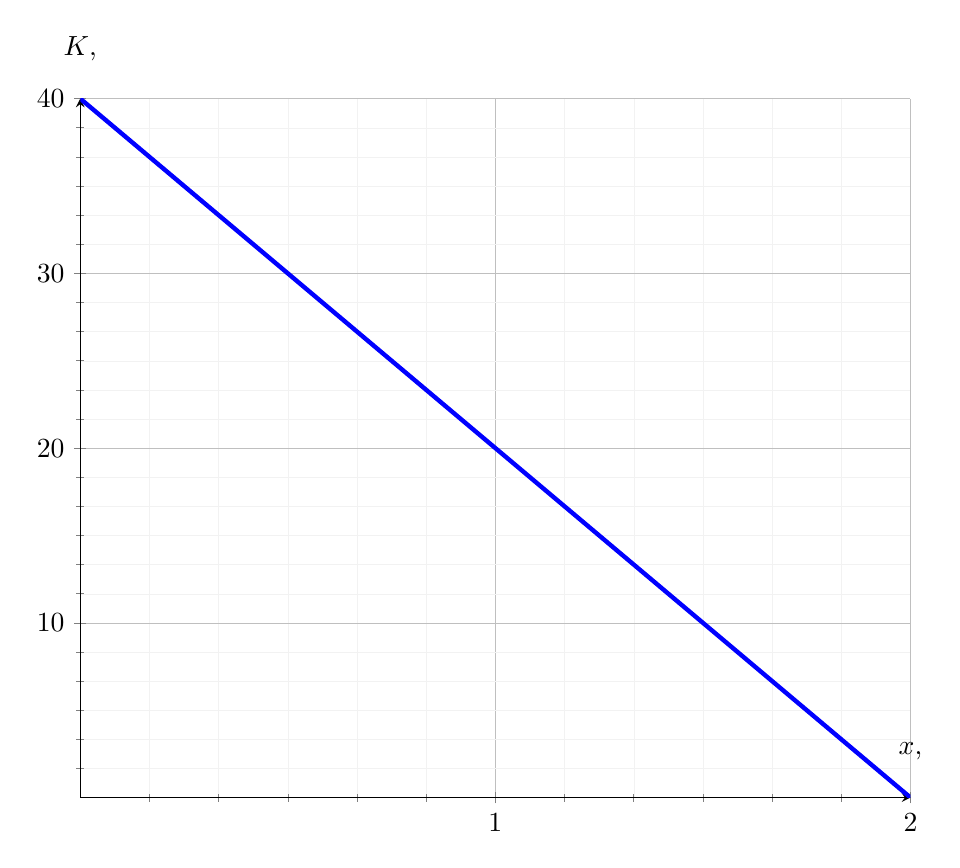
\begin{tikzpicture}[baseline]
		\begin{axis}[%
		% === Налаштування сітки ===
		grid = both,
		grid style={line width=.1pt, draw=gray!10},
		major grid style={line width=.2pt,draw=gray!50},
		minor tick num = 5,
		minor grid style = {line width=.1pt,draw=gray!10},
		% === Налаштування положення координатних осей ===
		axis lines = middle,
		axis line style={-stealth},
		% === Вибір підписів шкали для відображення ===
		xtick = {0,1,2},
		ytick = {0,10,...,40},
		% === Підпис координатних осей ===
		xlabel={$x$, \si{\meter}},
		ylabel={$K$, \si{\joule}},
		% === Положення підпису координатних осей ===
		xlabel style={above = 10pt},
		ylabel style={above = 10pt},
		% === Налаштування мінімальних та максимальних значень координат ===
		xmin = 0,
		xmax =  2,
		ymin = 0,
		ymax =  40,
		% === Налаштування розміру графіка ===
		width=\linewidth,
		]
		\addplot+[blue, no marks, domain={0:3}, samples=100, ultra thick] {40- 20*x};
		\end{axis}
		\end{tikzpicture}
		\caption{Problem~\ref{prb:ke_block_in_ramp}}
		\label{ke_block_in_ramp}
	\end{minipage}
	%---------------------------------------------------------
		\begin{minipage}[t]{0.45\linewidth}\centering
		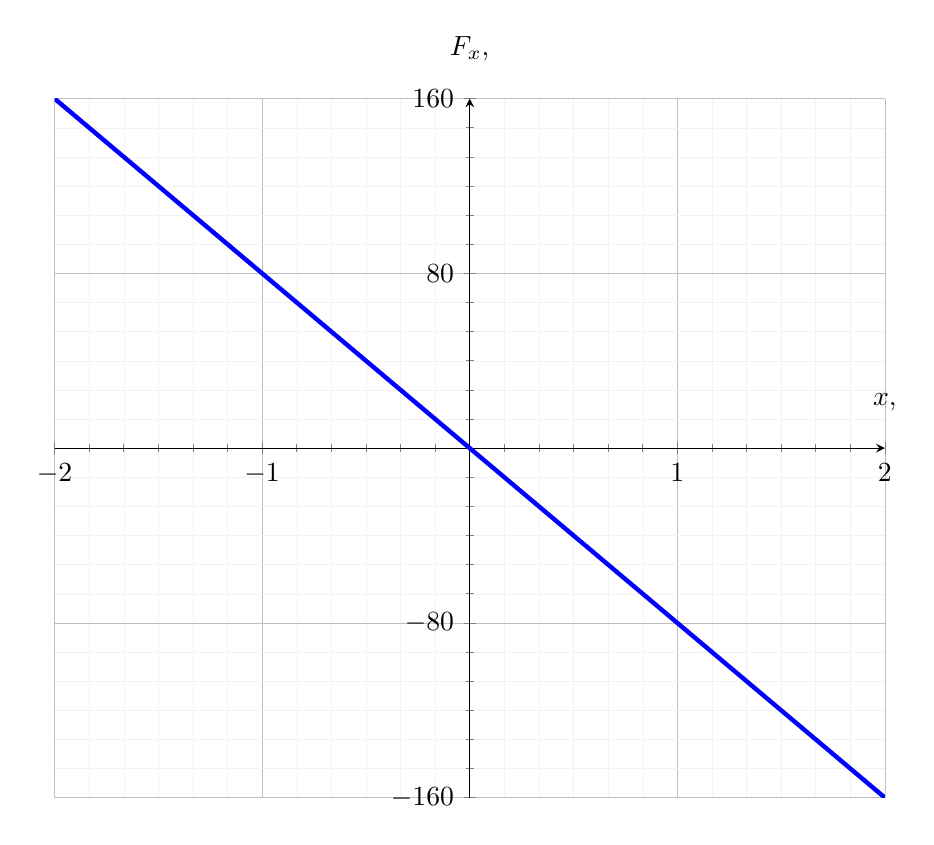
\begin{tikzpicture}[baseline]
		\begin{axis}[%
		% === Налаштування сітки ===
		grid = both,
		grid style={line width=.1pt, draw=gray!10},
		major grid style={line width=.2pt,draw=gray!50},
		minor tick num = 5,
		minor grid style = {line width=.1pt,draw=gray!10},
		% === Налаштування положення координатних осей ===
		axis lines = middle,
		axis line style={-stealth},
		% === Вибір підписів шкали для відображення ===
		xtick = {-2,-1,...,2},
		ytick = {-160,-80,...,160},
		% === Підпис координатних осей ===
		xlabel={$x$, \si{\meter}},
		ylabel={$F_x$, \si{\newton}},
		% === Положення підпису координатних осей ===
		xlabel style={above = 10pt},
		ylabel style={above = 10pt},
		% === Налаштування мінімальних та максимальних значень координат ===
		xmin = -2,
		xmax =  2,
		ymin = -160,
		ymax =  160,
		% === Налаштування розміру графіка ===
		width=\linewidth,
		]
		\addplot+[blue, no marks, domain={-2:2}, samples=100, ultra thick] {- 80*x};
	\end{axis}
	\end{tikzpicture}
	\vspace*{1.5ex}
	\caption{Problem~\ref{prb:w_force_vs_x}}
	\label{w_force_vs_x}
	\end{minipage}
	%---------------------------------------------------------
\end{figure}
%=========================================================


%=========================================================
\begin{problem}
	The kinetic energy of a particle moving along a circle of radius $R$ depends on the distance covered $s$ as $K = \alpha s^2$, a constant. Find the force acting on the particle as a function of $s$.
	\begin{solution}
		$F = 2\alpha s \sqrt{1 + (\nfrac{r}{R})^2}$.
	\end{solution}
\end{problem}



%=========================================================
\begin{problem}\label{prb:w_brick}
	A $10$~kg brick moves along an $x$ axis. Its acceleration as a function of its position is shown in Fig.~\ref{w_brick}. What is the net work performed on the brick by the force causing the acceleration as the brick moves from $x = 0$ to $x = 8.0$~m?
\end{problem}


%=========================================================
\begin{problem}\label{prb:ke_force_vs_x}
	The only force acting on a $2.0$~kg body as the body moves along an $x$ axis varies as shown in Fig.~\ref{ke_force_vs_x}. The velocity of the body at $x = 0$ is $4.0$~m/s. 
	\begin{enumerate*}[label=(\alph*)]
		\item What is the kinetic energy of the body at $x = 3.0$~m?
		\item At what value of x will the body have a kinetic energy of $8.0$~J?
		\item What is the maximum kinetic energy of the body between $x = 0$ and $x = 5.0$~m?
	\end{enumerate*}
\end{problem}

%=========================================================
\begin{figure}[h!]\centering
	%---------------------------------------------------------
	\begin{minipage}[t]{0.45\linewidth}\centering
		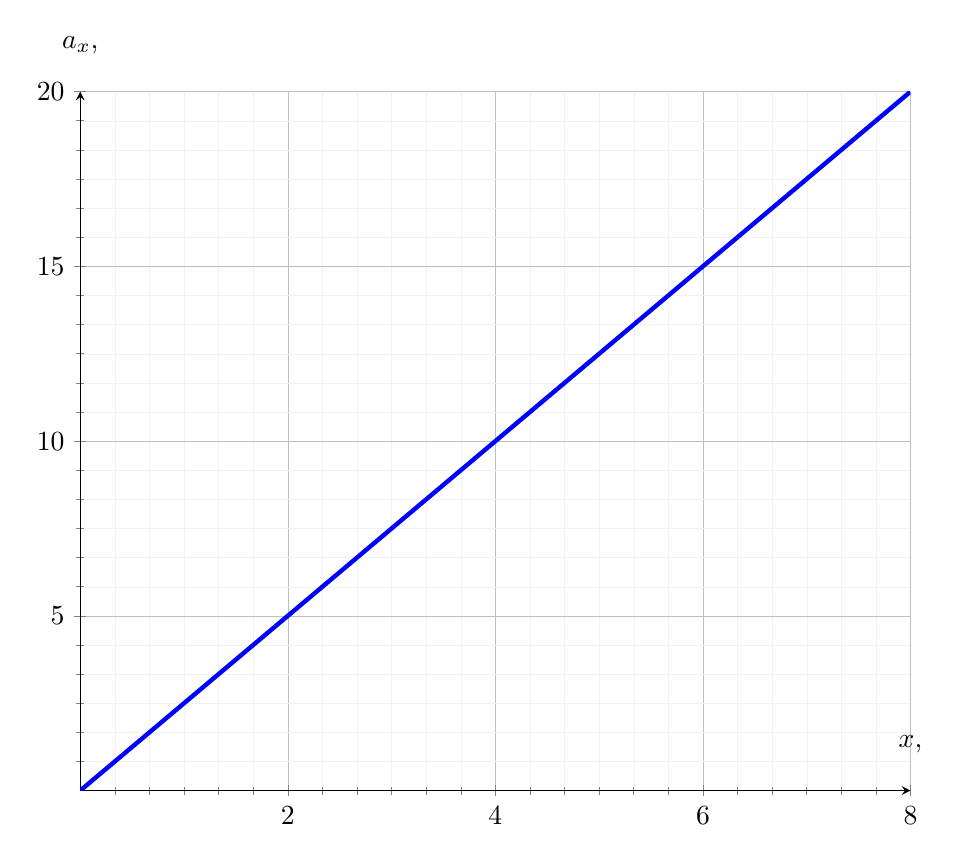
\begin{tikzpicture}[baseline]
			\begin{axis}[%
			% === Налаштування сітки ===
			grid = both,
			grid style={line width=.1pt, draw=gray!10},
			major grid style={line width=.2pt,draw=gray!50},
			minor tick num = 5,
			minor grid style = {line width=.1pt,draw=gray!10},
			% === Налаштування положення координатних осей ===
			axis lines = middle,
			axis line style={-stealth},
			% === Вибір підписів шкали для відображення ===
			xtick = {0,2,...,8},
			ytick = {0,5,...,20},
			% === Підпис координатних осей ===
			xlabel={$x$, \si{\meter}},
			ylabel={$a_x$, \si{\meter\per\square\second}},
			% === Положення підпису координатних осей ===
			xlabel style={above = 10pt},
			ylabel style={above = 10pt},
			% === Налаштування мінімальних та максимальних значень координат ===
			xmin = 0,
			xmax =  8,
			ymin = 0,
			ymax =  20,
			% === Налаштування розміру графіка ===
			width=\linewidth,
			]
			\addplot+[blue, no marks, domain={0:8}, samples=100, ultra thick] {20/8*x};
			\end{axis}
			\end{tikzpicture}
			\caption{Problem~\ref{prb:w_brick}}
			\label{w_brick}
	\end{minipage}
	%---------------------------------------------------------
	\begin{minipage}[t]{0.45\linewidth}\centering
		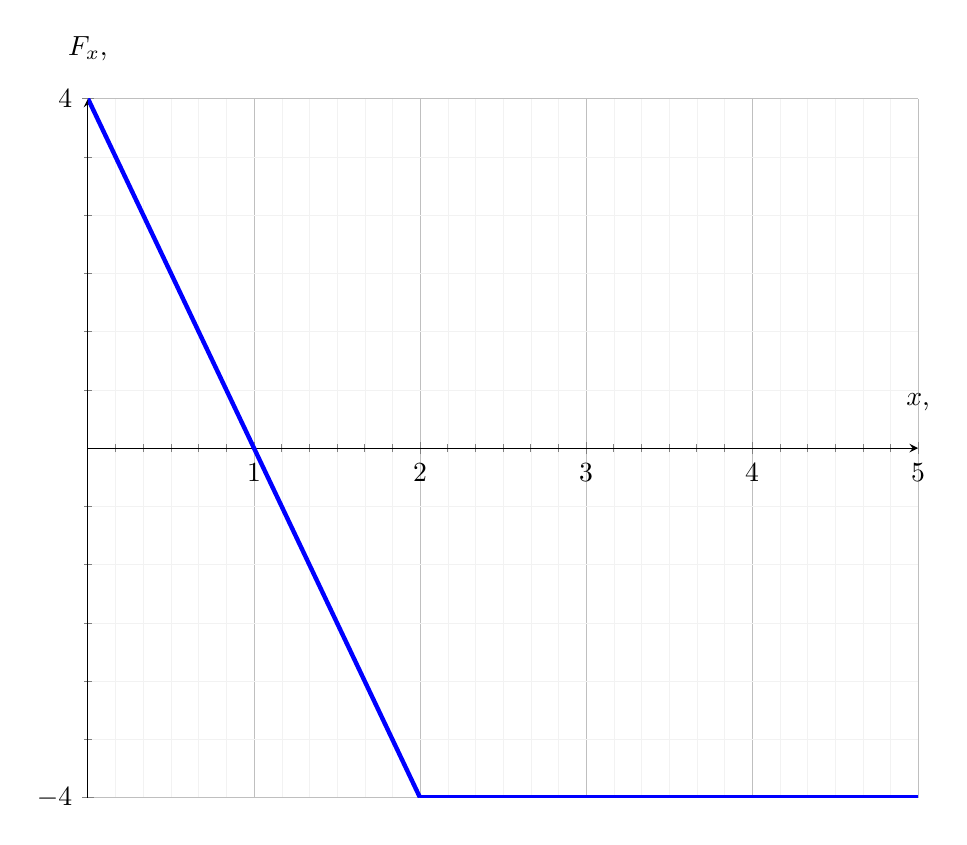
\begin{tikzpicture}[baseline]
			\begin{axis}[%
			% === Налаштування сітки ===
			grid = both,
			grid style={line width=.1pt, draw=gray!10},
			major grid style={line width=.2pt,draw=gray!50},
			minor tick num = 5,
			minor grid style = {line width=.1pt,draw=gray!10},
			% === Налаштування положення координатних осей ===
			axis lines = middle,
			axis line style={-stealth},
			% === Вибір підписів шкали для відображення ===
			xtick = {0,1,...,5},
			ytick = {-4,0,4},
			% === Підпис координатних осей ===
			xlabel={$x$, \si{\meter}},
			ylabel={$F_x$, \si{\newton}},
			% === Положення підпису координатних осей ===
			xlabel style={above = 10pt},
			ylabel style={above = 10pt},
			% === Налаштування мінімальних та максимальних значень координат ===
			xmin = 0,
			xmax =  5,
			ymin = -4,
			ymax =  4,
			% === Налаштування розміру графіка ===
			width=\linewidth,
			]
			\addplot+[blue, no marks, domain={0:2}, samples=100, ultra thick] {4-4*x};
			\addplot+[blue, no marks, domain={2:5}, samples=100, ultra thick] {-4};
			\end{axis}
		\end{tikzpicture}
		\vspace*{0.6ex}
		\caption{Problem~\ref{prb:ke_force_vs_x}}
		\label{ke_force_vs_x}
	\end{minipage}
	%---------------------------------------------------------
\end{figure}
%=========================================================


%=========================================================
\begin{problem}
	A disc of mass $m = 50$~g slides with the zero initial velocity down an inclined plane set at an angle $\theta = \ang{30}$ to the horizontal; having traversed the distance $l = 50$~cm along the horizontal plane, the disc stops. Find the work performed by the friction forces over the whole distance, assuming the friction coefficient $\mu = 0.15$ for both inclined and horizontal planes.
	\begin{solution}
		$W = -\frac{\mu mg l}{1 - \mu \cot\theta} = -0.05\,\si{\joule}$.
	\end{solution}
\end{problem}

%=========================================================
\begin{problem}
	The force on a particle is directed along an $x$ axis and given by $F = F_0(x/x_0 - 1)$. Find the work done by the force in moving the particle from $x = 0$ to $x = 2x_0$ by 
	\begin{enumerate*}[label=(\alph*)]
		\item plotting $F(x)$ and measuring the work from the graph and
		\item integrating F(x).
	\end{enumerate*}
	\begin{solution}
		$W = 0$.
	\end{solution}
\end{problem}


%=========================================================
\begin{problem}
	An initially stationary $2.0$~kg object accelerates horizontally and uniformly to a speed of $10$~m/s in $3.0$~s.
	\begin{enumerate*}[label=(\alph*)]
		\item In that $3.0$~s interval, how much work is done on the object by the force accelerating it? What is the instantaneous power due to that force
		\item at the end of the interval and
		\item at the end of the first half of the interval?
	\end{enumerate*}
\end{problem}

\section{Potential Energy}


%=========================================================
\begin{problem}\label{prb:pe_ball_on_rod}
	Figure~\ref{pe_ball_on_rod} shows a ball with mass $m = 0.341$~kg attached to the end of a thin rod with length $l = 0.452$~m and negligible mass. The other end of the rod is pivoted so that the ball can move in a vertical circle. The rod is held horizontally as shown and then given enough of a downward push to cause the ball to swing down and around and just reach the vertically up position, with zero speed there. How much work is done on the ball by the gravitational force from the initial point to 
	\begin{enumerate*}[label=(\alph*)]
		\item the lowest point,
		\item the highest point, and
		\item the point on the right level with the initial point? If the gravitational potential energy of the ball–Earth system is taken to be zero at the initial point, what is it when the ball reaches
		\item  the lowest point,
		\item the highest point, and
		\item the point on the right level with the initial point? 
%		\item Suppose the rod were pushed harder so that the ball passed through the highest point with a nonzero speed. Would $\Delta U_g$ from the lowest point to the highest point
%		then be greater than, less than, or the same as it was when the ball stopped at the highest point?
	\end{enumerate*}
\end{problem}


%=========================================================
\begin{problem}\label{prb:pe_loop-the-loop}
	In Fig.~\ref{pe_loop-the-loop} a small block of mass $m = 0.032$~kg can slide along the frictionless loop-the-loop, with loop radius $R = 12$~cm. The block is released from rest at point $P$, at height $h = 5.0R$ above the bottom of the loop. How much work does the gravitational force do on the block as the block travels from point $P$ to
	\begin{enumerate*}[label=(\alph*)]
		\item \label{pe_loop-the-loop_a} point $Q$ and
		\item the top of the loop?
		If the gravitational potential energy of the block–Earth system is taken to be zero at the bottom of the loop, what is that potential energy when the block is
		\item at point $P$,
		\item at point $Q$, and
		\item \label{pe_loop-the-loop_e} at the top of the loop?
	\end{enumerate*}
\end{problem}

%=========================================================
\begin{figure}[h!]\centering
	%---------------------------------------------------------
	\begin{minipage}[t]{0.45\linewidth}\centering
		\begin{tikzpicture}
			\pgfmathsetmacro{\R}{3}
			\draw[ultra thick, red, decoration={markings,mark= at position 0.5 with 
				{\arrow{latex};}},
				postaction=decorate, 
			] (0,0) +(-180:\R) arc (-180:90:\R);
			\draw[ultra thick, cyan] (0,0) -- node[above] {$l$} (180:\R) coordinate (B1);
			\draw[ball color = red!50] (B1) circle (0.5);
			\draw[ultra thick, cyan] (0,0) -- (90:\R) coordinate (B2);
			\draw[ball color = red!50 ,opacity=0.5] (B2) circle (0.5);
		\end{tikzpicture}
		\caption{Problem~\ref{prb:pe_ball_on_rod}}
		\label{pe_ball_on_rod}
	\end{minipage}
	%---------------------------------------------------------
	\begin{minipage}[t]{0.45\linewidth}\centering
		\begin{tikzpicture}
			\tikzset{
				body/.pic = {
					\draw[black, fill=red!50] (0,-0.25) rectangle (0.5,0.25);
				}
			}
			\pgfmathsetmacro{\R}{2}
			\tikzstyle{ground}=[fill,pattern=north east lines,draw=none,minimum width=8cm,minimum height=0.3cm]
			\node (wall) [ground, minimum width=8cm,yshift=-0.15cm] {};
			\draw (wall.north west) -- (wall.north east);
			\draw[ultra thick, cyan] (-3,10) coordinate (P) to[out=270, in = 180] (2,0);
			\draw[ultra thick, cyan] (2,\R) +(-90:\R) arc (-90:180:\R);
			\draw(-4,10) -- +(1,0);
			\draw[latex-latex]  (-3.5, 10) -- node[fill=white] {$h$} +(0,-10);
			\coordinate (Q) at (2+\R,\R);
			\draw[-latex] (2,\R) -- node[fill=white] {$R$} +(135:\R);
			\pic[] at (P) {body}; \node[right=0.5cm] at (P) {$P$};
			\pic[xshift=-0.5cm] at (Q) {body}; \node[right] at (Q) {$Q$};
		\end{tikzpicture}
		\caption{Problem~\ref{prb:pe_loop-the-loop}}
		\label{pe_loop-the-loop}
	\end{minipage}
	%---------------------------------------------------------
\end{figure}
%=========================================================


%=========================================================
\begin{problem}
	A locomotive of mass $m$ starts moving so that its velocity varies according to the law $v = \alpha\sqrt{s}$, where $\alpha$ is a constant, and $s$ is the distance covered. Find the total work performed by all the forces which are acting on the locomotive during the first $t$ seconds after the beginning of motion.
	\begin{solution}
		$W = \frac{m\alpha^4t^2}{8}$.
	\end{solution}
\end{problem}


\section{Conservation of Mechanical Energy of the Particle}


%=========================================================
\begin{problem}
	A $5.0$~g marble is fired vertically upward using a spring gun. The spring must be compressed $8.0$~cm if the marble is to just reach a target $20$~m above the marble's position on the compressed spring. 
	\begin{enumerate*}[label=(\alph*)]
		\item What is the change $\Delta U_g$ in the gravitational potential energy of the marble–Earth system during the 20 m ascent? 
		\item What is the change in the elastic potential energy of the spring during its launch of the marble?
		\item What is the spring constant of the spring?
	\end{enumerate*}
\end{problem}


%=========================================================
\begin{problem}
	A pendulum consists of a $2.0$~kg stone swinging on a $4.0$~m string of negligible mass. The stone has a speed of $8.0$~m/s when it passes its lowest point. 
	\begin{enumerate*}[label=(\alph*)]
		\item What is the speed when the string is at $\ang{60}$ to the vertical?
		\item  What is the greatest angle with the vertical that the string will reach during the stone’s motion?
		\item If the potential energy of the pendulum–Earth system is taken to be zero at the stone’s lowest point, what is the total mechanical energy of the system?
	\end{enumerate*}
\end{problem}


%=========================================================
\begin{problem}\label{prb:ce_ball_on_string}
	The string in Fig.~\ref{ce_ball_on_string} is $l = 120$~cm long, has a ball attached to one end, and is fixed at its other end. The distance $d$ from the fixed end to a fixed peg at point $P$ is $75.0$~cm. When the initially stationary ball is released with the string horizontal as shown, it will swing along the dashed arc. What is its speed when it reaches 
	\begin{enumerate*}[label=(\alph*)]
		\item its lowest point and
		\item its highest point after the string catches on the peg?
	\end{enumerate*}
\end{problem}


%---------------------------------------------------------
\begin{figure}[h!]\centering
	\begin{tikzpicture}
	\pgfmathsetmacro{\l}{6}
	\pgfmathsetmacro{\d}{3}
	\draw[ultra thick, red, dashed, decoration={markings,mark= at position 0.5 with 
		{\arrow{latex};}},
	postaction=decorate, 
	] (0,0) +(180:\l) arc(180:270:\l);
	\node[right] at (0,0) {$O$};
	\draw (0,0) -- node[above] {$l$} +(180:\l) coordinate (P1);
	\draw[ball color = red!50] (P1) circle (0.5);
	\draw (0,0) -- +(270:\l) coordinate (P2);
	\draw[ball color = red!50] (P2) circle (0.5);
	\coordinate (P) at (0,-\d); \node[right] at (P) {$P$};
	\draw[ultra thick, red, dashed, decoration={markings,mark= at position 0.5 with 
		{\arrow{latex};}},
	postaction=decorate, 
	] (P) +(270:{\l-\d}) arc (270:360:{\l-\d});	
	\draw[-latex] (P) -- node[fill=white] {$r$}+(-45:{\l-\d});
	\draw[fill=cyan] (0,0) circle (0.1);
	\draw[fill=cyan] (P) circle (0.1);
	\end{tikzpicture}
	\caption{Problem~\ref{prb:ce_ball_on_string}}
	\label{ce_ball_on_string}
\end{figure}
%---------------------------------------------------------

\section{Relationship Between Conservative. Forces and Potential Energy Reading a Potential Energy Curve}


%=========================================================
\begin{problem}
	The potential energy of a system of two particles
	separated by a distance r is given by $U(r) = \frac{A}{r}$, where $A$ is a constant. Find the radial force $\vec F_r$ that each particle exerts on the other.
	\begin{solution}
		$\frac{A}{r^2}$a way from the other particle.
	\end{solution}
\end{problem}



%=========================================================
\begin{problem}
	A potential energy function for a system in which a two dimensional
	force acts is of the form $U = 3x^33y - 7x$. Find the force that acts at the point $(x, y)$.
\end{problem}


%=========================================================
\begin{problem}\label{prb:pe_U_vs_x}
	\addpic{2}{0.5\linewidth}{%
	%---------------------------------------------------------
	\begin{tikzpicture}[baseline]
		\begin{axis}[%
		% === Налаштування сітки ===
		grid = both,
		grid style={line width=.1pt, draw=gray!10},
		major grid style={line width=.2pt,draw=gray!50},
		minor tick num = 5,
		minor grid style = {line width=.1pt,draw=gray!10},
		% === Налаштування положення координатних осей ===
		axis lines = middle,
		axis line style={-stealth},
		% === Вибір підписів шкали для відображення ===
		xtick = {2,4,5,6,7},
		ytick = {0,15,35,45},
		% === Підпис координатних осей ===
		xlabel={$x$, \si{\meter}},
		ylabel={$U$, \si{\joule}},
		% === Положення підпису координатних осей ===
		xlabel style={above = 10pt},
		ylabel style={above = 10pt},
		% === Налаштування мінімальних та максимальних значень координат ===
		xmin = 0,
		xmax =  7,
		ymin = 0,
		ymax =  45,
		% === Налаштування розміру графіка ===
		width=\linewidth,
		]
		\addplot+[blue, no marks, domain={0:2}, samples=100, ultra thick] {35};
		\addplot+[blue, no marks, domain={2:4}, samples=100, ultra thick] {-10*x+55};
		\addplot+[blue, no marks, domain={4:5}, samples=100, ultra thick] {15};
		\addplot+[blue, no marks, domain={5:6}, samples=100, ultra thick] {30*x -135};
		\addplot+[blue, no marks, domain={6:7}, samples=100, ultra thick] {45};
		\end{axis}
	\end{tikzpicture}
	\captionof{figure}{Problem~\ref{prb:pe_U_vs_x}}
	\label{pe_U_vs_x}	
	%---------------------------------------------------------
}[7]%	
	Figure~\ref{pe_U_vs_x} shows a plot of potential energy $U$ versus position $x$ of a $0.90$~kg particle that can travel only along an $x$ axis. (Nonconservative forces are not involved.) The particle is released at $x = 4.5$~m with an initial velocity of $7.0$~m/s, headed in the negative $x$ direction. 
	\begin{enumerate*}[label=(\alph*)]
		\item If the particle can reach $x = 1.0$~m, what is its velocity there, and if it cannot, what is its turning point?
		What are the
		\item magnitude and
		\item  direction of the force on the particle as it begins to move to the left of $x = 4.0$~m?
		Suppose, instead, the particle is headed in the positive $x$ direction when it is released at $x = 4.5$~m at speed $7.0$~m/s.
		\item If the particle can reach $x = 7.0$~m, what is its speed there, and if it cannot, what is its turning point?
		What are the
		\item magnitude and
		\item direction of the force on the particle as it begins to move to the right of $x = 5.0$~m?
	\end{enumerate*}
	\begin{solution}
		\begin{enumerate*}[label=(\alph*)]
			\item $2.1$~m/s;
			\item $10$~N;
			\item $+x$ direction;
			\item $5.7$~m;
			\item $30$~N;
			\item $-x$ direction.
		\end{enumerate*}
	\end{solution}
\end{problem}


%=========================================================
\begin{problem}
	The potential energy of a diatomic molecule (a two-atom system like \ce{H2} or \ce{O2}) is given by 
	\[
		U = \frac{a}{r^{12}} - \frac{b}{r^6}
	\]
	where $r$ is the separation of the two atoms of the molecule and $a$ and $b$ are positive constants. This potential energy is associated with the force that binds the two atoms together.
	\begin{enumerate*}[label=(\alph*)]
		\item Find the equilibrium separation --- that is, the distance between the atoms at which the force on each atom is zero.
		Is the force repulsive (the atoms are pushed apart) or attractive (they are pulled together) if their separation is
		\item smaller and
		\item larger than the equilibrium separation?
	\end{enumerate*} 
\end{problem}


\section{Center of Mass. Law for a System of Particles and Linear Momentum Conservation Law}

%=========================================================
\begin{problem}\label{prb:cm_three_balls}
	\addpic{1}{0.5\linewidth}{%
			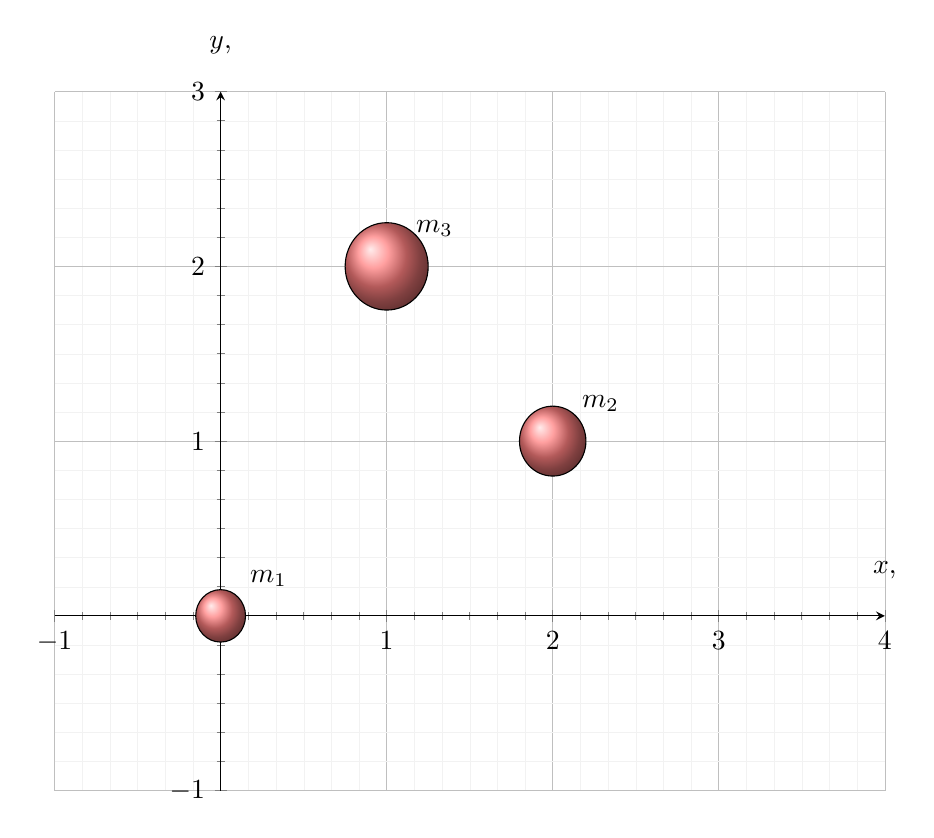
\begin{tikzpicture}[baseline]
			\begin{axis}[%
			% === Налаштування сітки ===
			grid = both,
			grid style={line width=.1pt, draw=gray!10},
			major grid style={line width=.2pt,draw=gray!50},
			minor tick num = 5,
			minor grid style = {line width=.1pt,draw=gray!10},
			% === Налаштування положення координатних осей ===
			axis lines = middle,
			axis line style={-stealth},
			% === Вибір підписів шкали для відображення ===
			xtick = {-1,0,...,4},
			ytick = {-1,0,...,3},
			% === Підпис координатних осей ===
			xlabel={$x$, \si{\meter}},
			ylabel={$y$, \si{\meter}},
			% === Положення підпису координатних осей ===
			xlabel style={above = 10pt},
			ylabel style={above = 10pt},
			% === Налаштування мінімальних та максимальних значень координат ===
			xmin = -1,
			xmax =  4,
			ymin = -1,
			ymax =  3,
			% === Налаштування розміру графіка ===
			width=\linewidth,
			]
			\draw[ball color = red!50] (axis cs:0,0) circle (0.15) node[above right=0.25cm] {$m_1$}; 
			\draw[ball color = red!50] (axis cs:1,2) circle (0.25) node[above right=0.25cm] {$m_3$}; 
			\draw[ball color = red!50] (axis cs:2,1) circle (0.2)  node[above right=0.25cm] {$m_2$}; 
			\end{axis}
			\end{tikzpicture}
			\captionof{figure}{Problem~\ref{prb:cm_three_balls}}
			\label{cm_three_balls}
	}%  
	Figure~\ref{cm_three_balls} shows a three-particle system, with masses $m_1 = 3.0$~kg, $m_2 = 4.0$~kg, and $m_3 = 8.0$~kg. What are 
	\begin{enumerate*}[label=(\alph*)]
		\item the $x$ coordinate and
		\item the $y$ coordinate of the system’s center of mass?
		\item If $m_3$ is gradually increased, does the center of mass of the system shift toward or away from that particle, or does it remain stationary?
	\end{enumerate*}
\end{problem}

%=========================================================
\begin{problem}
	 \correct{0.5\linewidth}[6]%
	A stone is dropped at $t = 0$. A second stone, with twice the mass of the first, is dropped from the same point at $t = 100$~ms. 
	\begin{enumerate*}[label=(\alph*)]
		\item How far below the release point is the center of mass of the two stones at $t = 300$~ms? (Neither stone has yet reached the ground.)
		\item How fast is the center of mass of the twostone system moving at that time?
	\end{enumerate*}
	\begin{solution}
		\begin{enumerate*}[label=(\alph*)]
			\item $28$~cm;
			\item $2.3$~m/s.
		\end{enumerate*}
	\end{solution}
\end{problem}

%=========================================================
\begin{problem}\label{prb:cm_two_part}
	\addpic{1}{5.5cm}{%
	\begin{tikzpicture}
		\pgfmathsetmacro{\l}{2}
		\pgfmathsetmacro{\lang}{45}
		\node (wall) [ground, minimum width=5cm,yshift=-0.25cm] at (2.5,0) {};
		\draw (wall.north west) -- (wall.north east);
		\draw [-latex] (0,0) -- +(0,2.5) node[above] {$y$};
		\draw [-latex] (0,0) -- +(5,0) node[above] {$x$};
		\draw [dashed] (0,0) --+(\lang:{\l/cos(\lang)}) coordinate (B2);
		\draw [-latex] (B2) node[above] {$2$} -- +(\lang:0.5);
		\draw [ball color=blue!50] (B2) circle (0.1);
		\coordinate (B1) at (\l,0.2); 
		\draw [ball color=blue!50, -latex] (B1) -- +(0.5,0);
		\draw [ball color=red!50]  (B1) node[above] {$1$} circle (0.1);
		\end{tikzpicture}
		\captionof{figure}{Problem~\ref{prb:cm_two_part}}
		\label{cm_two_part}
		}[3]%  
	In Figure~\ref{cm_two_part}, two particles are launched from the origin of the coordinate system at time $t = 0$. Particle 1 of mass $m_1 = 5.00$~g is shot directly along the $x$ axis on a frictionless floor, with constant speed $10.0$~m/s. Particle 2 of mass $m_2 = 3.00$~g is shot with a velocity of magnitude $20.0$~m/s, at an upward angle such that it always stays directly above particle 1. 
	\begin{enumerate*}[label=(\alph*)]
		\item What is the maximum height $h_{\max}$ reached by the com of the two-particle system? 
		In unit-vector notation, what are the
		\item velocity and 
		\item acceleration of the com when the com reaches~$h_{\max}$?
	\end{enumerate*}
\end{problem}

%=========================================================
\begin{problem}
	A shell is shot with an initial velocity $\vec v_0$ of magnitude $20$~m/s, at an angle $\alpha = \ang{60}$ of with the horizontal. At the top of the trajectory, the shell explodes into two fragments of equal mass. One fragment, whose velocity immediately after the explosion is zero, falls vertically. How far from the gun does the other fragment land, assuming that the terrain is level and that air drag is negligible?
	\begin{solution}
		$53$~m.
	\end{solution}
\end{problem}

%=========================================================
\begin{problem}
	A $0.30$~kg softball has a velocity of $15$~m/s at an angle of \ang{35} below the horizontal just before making contact with the bat. What is the magnitude of the change in momentum of the ball while in contact with the bat if the ball leaves with a velocity of 
	\begin{enumerate*}[label=(\alph*)]
		\item $20$~m/s, vertically downward, and
		\item horizontally back toward the pitcher?
	\end{enumerate*}
	\begin{solution}
		\begin{enumerate*}[label=(\alph*)]
			\item $5.0$~\si{\kilo\gram\meter\per\second};
			\item  $10.0$~\si{\kilo\gram\meter\per\second}.
		\end{enumerate*}
	\end{solution}
\end{problem}


%=========================================================
\begin{problem}
	The vector position of a particle of mass $3.50$~g  moving in the $xy$ plane varies in time according to $\vec r = 3\vec i + (3 t +2t^2) \vec j$, where $t$ is in seconds and $\vec r_1$ is in centimeters. At the same time, the vector position of a  particle of mass $5.50$~g varies as $(3-2t^2) \vec i 6t \vec j$. At $t = 2.50$~s, determine
	\begin{enumerate*}[label=(\alph*)]
		\item the vector position of the center of mass,
		\item the linear momentum of the system,
		\item the velocity of the center of mass,
		\item the acceleration of the center of mass,
		and
		\item the net force exerted on the two-particle system.
	\end{enumerate*}
	\begin{solution}
		
	\end{solution}
\end{problem}


%=========================================================
\begin{problem}
	An object, with mass $m$ and speed $v$ relative to an observer, explodes into two pieces, one three times as massive as the other; the explosion takes place in deep space. The less massive piece stops relative to the observer. How much kinetic energy is added to the system during the explosion, as measured in the observer’s reference frame?
\end{problem}

%=========================================================
\begin{problem}
	A $20.0$~kg body is moving through space in the positive direction of an $x$ axis with a speed of $200$~m/s when, due to an internal explosion, it breaks into three parts. One part, with a mass of $10.0$~kg, moves away from the point of explosion with a speed of $100$~m/s in the positive $y$ direction. A second part, with a mass of $4.00$~kg, moves in the negative $x$ direction with a speed of $500$~m/s. 
	\begin{enumerate*}[label=(\alph*)]
		\item In unit-vector notation, what is the velocity of the third part?
		\item How much energy is released in the explosion? Ignore effects due to the gravitational force.
	\end{enumerate*}
	\begin{solution}
		\begin{enumerate*}[label=(\alph*)]
			\item $(1.00 \vec i - 0.167\vec j)$~km/s; 
			\item $3.23$~MJ.
		\end{enumerate*}
	\end{solution}
\end{problem}

%=========================================================
\begin{problem}
	A $4.0$~kg mess kit sliding on a frictionless surface explodes into two $2.0$~kg parts: $3.0$~m/s, due north, and $5.0$~m/s, \ang{30} north of east. What is the original speed of the mess kit?
\end{problem}

%=========================================================
\begin{problem}
	A vessel at rest at the origin of an $xy$ coordinate system explodes into three pieces. Just after the explosion, one piece, of mass $m$, moves with velocity ($-30$~m/s) and a second piece, also of mass m, moves with velocity ($-30$~m/s). The third piece has mass $3m$. Just after the explosion, what are the 
	\begin{enumerate*}[label=(\alph*)]
		\item magnitude and
		\item direction of the velocity of the third piece?
	\end{enumerate*}
	\begin{solution}
		\begin{enumerate*}[label=(\alph*)]
			\item $14$~m/s;
			\item \ang{45}.
		\end{enumerate*}
	\end{solution}
\end{problem}


%=========================================================
\begin{problem}
	Particle A and particle B are held together with a compressed spring between them. When they are released, the spring pushes them apart, and they then fly off in opposite directions, free of the spring. The mass of A is $2.00$ times the mass of B, and the energy stored in the spring was $60$~J. Assume that the spring has negligible mass and that all its stored energy is transferred to the particles. Once that transfer is complete, what are the kinetic energies of 
	\begin{enumerate*}[label=(\alph*)]
		\item particle A and
		\item particle B?
	\end{enumerate*}
\end{problem}

\section{Equation of motion of a body with a variable mass}


%=========================================================
\begin{problem}
	A model rocket engine has an average thrust of $5.26$~N. It has an initial mass of $25.5$~g, which includes fuel mass of $12.7$~g. The duration of its burn is $1.90$~s.
	\begin{enumerate*}[label=(\alph*)]
		\item What is the average exhaust speed of the engine?
		\item This engine is placed in a rocket body of mass $53.5$~g.
	\end{enumerate*}
	 What is the final velocity of the rocket if it were to be fired from rest in outer space by an astronaut on a spacewalk? Assume the fuel burns at a constant rate.
	\begin{solution}
		\begin{enumerate*}[label=(\alph*)]
			\item $787$~m/s; 
			\item $138$~m/s.
		\end{enumerate*}
	\end{solution}
\end{problem}


%=========================================================
\begin{problem}
	A $6090$~kg space probe moving nose-first toward Jupiter at $105$~m/s relative to the Sun fires its rocket engine, ejecting $80.0$~kg of exhaust at a speed of $253$~m/s relative to the space probe.What is the final velocity of the probe?
\end{problem}


%=========================================================
\begin{problem}
	A rocket that is in deep space and initially at rest relative to an inertial reference frame has a mass of $2.55 \cdot 10^5$~kg, of which $1.81  \cdot 10^5$~kg is fuel. The rocket engine is then fired for $250$~s while fuel is consumed at the rate of $480$~kg/s. The speed of the exhaust products relative to the rocket is $3.27$~km/s. 
	\begin{enumerate*}[label=(\alph*)]
		\item What is the rocket’s thrust? After the $250$~s firing,
		what are
		\item the mass 
		and
		\item the speed of the rocket?
	\end{enumerate*}
	\begin{solution}
		\begin{enumerate*}[label=(\alph*)]
			\item $1.57 \cdot 10^6$~N;
			\item $1.35 \cdot 10^5$~kg; 
			\item $2.08$~km/s.
		\end{enumerate*}
	\end{solution}
\end{problem}



\section{Collisions of Particles}

\subsection{Momentum and Kinetic Energy in Collisions}

%=========================================================
\begin{problem}
	A $1.2$~kg ball drops vertically onto a floor, hitting with a speed of $25$~m/s. It rebounds with an initial speed of $10$~m/s.
	\begin{enumerate*}[label=(\alph*)]
		\item What impulse acts on the ball during the contact?
		\item If the ball is in contact with the floor for 0.020 s, what is the magnitude of the average force on the floor from the ball?
	\end{enumerate*}
	\begin{solution}
		\begin{enumerate*}[label=(\alph*)]
			\item $42$~\si{\newton\second};
			\item $2.1$~kN
		\end{enumerate*}
	\end{solution}
\end{problem}

%=========================================================
\begin{problem}
	A particle of mass $m$ having collided with a stationary particle of mass $M$ deviated by an angle $\nfrac{\pi}{2}$ whereas the particle $M$ recoiled at an angle $\theta = \ang{30}$ to the direction of the initial motion of the particle $m$. How much (in per cent) and in what way has the kinetic energy of this system changed after the collision, if $\nfrac{M}{m} = 5.0$?
	\begin{solution}
		$40\%$.
	\end{solution}
\end{problem}


%=========================================================
\begin{problem}
	A bullet of mass $10$~g strikes a ballistic pendulum of mass $2.0$~kg.The center of mass of the pendulum rises a vertical distance of $12$~cm. Assuming that the bullet remains embedded in the pendulum, calculate the bullet's initial speed.
	\begin{solution}
		$3.1 \cdot 10^2$~m/s.
	\end{solution}
\end{problem}

%=========================================================
\begin{problem}
	A $3.50$~g bullet is fired horizontally at two blocks at rest on a frictionless table. The bullet passes through block 1 (mass $1.20$~kg) and embeds itself in block 2 (mass $1.80$~kg). The blocks end up with speeds $v_1 = 0.630$~m/s and $v_2 = 1.40$~m/s. Neglecting the material removed from block 1 by the bullet, find the speed of the bullet as it 
	\begin{enumerate*}[label=(\alph*)]
		\item leaves and
		\item enters block 1.
	\end{enumerate*}
	\begin{solution}
	\begin{enumerate*}[label=(\alph*)]
		\item $721$~m/s; 
		\item $937$~m/s.
	\end{enumerate*}
	\end{solution}
\end{problem}

\subsection{Elastic Collisions in One Dimension}


%=========================================================
\begin{problem}
	A cart with mass $340$~g moving on a frictionless linear air track at an initial speed of $1.2$~m/s undergoes an elastic collision with an initially stationary cart of unknown mass. After the collision, the first cart continues in its original direction at $0.66$~m/s.
	\begin{enumerate*}[label=(\alph*)]
		\item What is the mass of the second cart? 
		\item What is its speed after impact?
		\item What is the speed of the twocart center of mass?
	\end{enumerate*}
	\begin{solution}
		\begin{enumerate*}[label=(\alph*)]
			\item $99$~g;
			\item $1.9$~m/s;
			\item $0.93$~m/s.
		\end{enumerate*}
	\end{solution}
\end{problem}

%=========================================================
\begin{problem}
	A body of mass $2.0$~kg makes an elastic collision with another body at rest and continues to move in the original direction but with one-fourth of its original speed.
	\begin{enumerate*}[label=(\alph*)]
		\item What is the mass of the other body?
		\item What is the speed of the two-body center of mass if the initial speed of the $2.0$~kg body was $4.0$~m/s? 
	\end{enumerate*}
	\begin{solution}
		\begin{enumerate*}[label=(\alph*)]
			\item $1.2$~kg; 
			\item $2.5$~m/s.
		\end{enumerate*}
	\end{solution}
\end{problem}


%=========================================================
\begin{problem}\label{prb:col_ball_hit_block}
	\addpic{0}{6cm}{%
			\begin{tikzpicture}
			\pgfmathsetmacro{\R}{0.4}
			\pgfmathsetmacro{\l}{3}
			\draw [fill=red!50] (2,0) rectangle +(1,1);
			\draw [ultra thick, cyan] ({2-\R},0.5) -- +(0,\l) coordinate(O);
			\draw [dashed, postaction=decorate, decoration={markings,mark= at position 0.5 with 
				{\arrow{latex};}},]
			(O) +(180:\l) arc(180:270:\l);
			\draw [ultra thick, cyan] (O) -- +(-\l,0) coordinate (S);
			\node[pt = red] at (O) {};
			\draw[ball color = blue] ({2-\R},0.5) circle (\R);
			\draw[ball color = blue] (S) circle (\R);
			\node (wall) [ground, minimum width=6cm,yshift=-0.68cm] at ({2-\R},0.5) {};
			\draw (wall.north west) -- (wall.north east);
			\end{tikzpicture}
			\captionof{figure}{Problem~\ref{prb:col_ball_hit_block}}
			\label{col_ball_hit_block}
		}[8]%
	A steel ball of mass $0.500$~kg is fastened to a cord that is $70.0$~cm long and fixed at the far end. The ball is then released when the cord is horizontal (Fig.~\ref{col_ball_hit_block}). At the bottom of its path, the ball strikes a $2.50$~kg steel block initially at rest on a frictionless surface. The collision is elastic. Find 
	\begin{enumerate*}[label=(\alph*)]
		\item the speed of the ball 
		and
		\item the speed of the block, both just after the collision.
	\end{enumerate*}
\end{problem}


\subsection{Collisions in Two Dimensions}


%=========================================================
\begin{problem}
	Ball B, moving in the positive direction of an $x$ axis at speed $v$, collides with stationary ball A at the origin. A and B have different masses. After the collision, B moves in the negative direction of the $y$ axis at speed $v/2$. 
	\begin{enumerate*}[label=(\alph*)]
		\item In what direction does A move?
		\item Show that the speed of A cannot be determined from the given information.
	\end{enumerate*}
\end{problem}


%=========================================================
\begin{problem}
	After a completely inelastic collision, two objects of the same
	mass and same initial speed move away together at half their initial
	speed. Find the angle between the initial velocities of the objects.
	\begin{solution}
		\ang{120}.
	\end{solution}
\end{problem}


%=========================================================
\begin{problem}
	A projectile proton with a speed of $500$~m/s collides elastically
	with a target proton initially at rest. The two protons then
	move along perpendicular paths, with the projectile path at \ang{60}
	from the original direction. After the collision, what are the speeds
	of 
	\begin{enumerate*}[label=(\alph*)]
		\item the target proton and
		\item the projectile proton?
	\end{enumerate*}
	\begin{solution}
		\begin{enumerate*}[label=(\alph*)]
			\item $433$ m/s; 
			\item $250$ m/s.
		\end{enumerate*}	
	\end{solution}
\end{problem}

%=========================================================
\begin{problem}\label{prb:col_three_balls}
	\addpic{2}{6cm}{%
			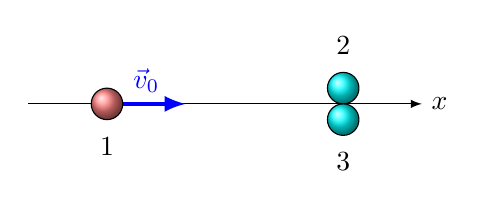
\begin{tikzpicture}
			\draw[-latex] (0,0) -- +(5,0) node[right] {$x$};
			\draw [ultra thick, blue, -latex] (1,0) -- node[above] {$\vec v_0$} +(1,0);
			\draw[ball color = red!50] (1,0) circle (0.2);
			\node[below=0.3cm] at (1,0) {$1$};
			\draw[ball color = cyan] (4,0.2) node[above=0.3cm] {$2$} circle (0.2);
			\draw[ball color = cyan] (4,-0.2) node[below=0.3cm] {$3$} circle (0.2);
			\end{tikzpicture}
			\captionof{figure}{Problem~\ref{prb:col_three_balls}}
			\label{col_three_balls}%
		}[2]%  
	The three balls in the overhead view of Fig.~\ref{col_three_balls} are identical. Balls 2 and 3 touch each other and are aligned perpendicular to the path of ball 1. The velocity of ball 1 has magnitude $v_0 = 10$~m/s and is directed at the contact point of balls 1 and 2. After the collision, what are the
	\begin{enumerate*}[label=(\alph*)]
		\item speed 
		and
		\item direction of the velocity of ball 2,
		\item the direction of the velocity of ball 2, 
		\item the speed 
		and
		\item direction of the velocity of ball 3, 
		and 
		\item the speed and
		\item direction of the velocity of ball 1? (Hint:With friction absent, each impulse is directed along the line connecting the centers of the colliding balls, normal to the colliding surfaces.)
	\end{enumerate*}
	\begin{solution}
		\begin{enumerate*}[label=(\alph*)]
			\item $6.9$~m/s;
			\item \ang{30};
			\item $6.9$~m/s;
			\item \ang{-30};
			\item $2.0$~m/s;
			\item \ang{180}.
		\end{enumerate*}
	\end{solution}
\end{problem}




\section{Angular Momentum and Torque}

%=========================================================
\begin{problem}
	A particle of mass $1.50$~kg moves in the $xy$ plane with a velocity of $\vec v = 4.20\vec i - 3.60\vec j$~m/s. Determine the angular momentum of the particle about the origin when its position vector is $\vec r = 1.50 \vec i + 2.20 \vec j$~m.
\end{problem}

%=========================================================
\begin{problem}
	At one instant, force $\vec F = 4.0 \vec j$~N acts on a $0.25$~kg object
	that has position vector $\vec r  = 2.0 \vec i - 2.0 \vec k$ (in meters) and velocity vector $\vec v = -5.0 \vec i + 5.0 \vec k$ (in \si{\meter\per\second}). About the origin and in unit-vector notation, what are 
	\begin{enumerate*}[label=(\alph*)]
		\item the object’s angular momentum and
		\item the torque acting on the object?
	\end{enumerate*}
	\begin{solution}
		\begin{enumerate*}[label=(\alph*)]
			\item 0; 
			\item $8.0 \vec i + 8.0 \vec k$ (in \si{\newton\meter}).
		\end{enumerate*}
	\end{solution}
\end{problem}

%=========================================================
\begin{problem}
	At the instant the displacement of a $2.00$~kg object relative to the origin is $\vec d = 2.00 \vec i + 4.00 \vec j -3.00 \vec k$ (in meters) its velocity is $\vec v  = -6.00 \vec i + 3.00\vec j + 3.00 \vec k$ (in \si{\meter\per\second}) and it is subject to a force $\vec F = 6.00 \vec i - 8.00 \vec j - 4.00 \vec k$. Find 
	\begin{enumerate*}[label=(\alph*)]
		\item the acceleration of the object,
		\item the angular momentum of the object about the origin,
		\item the torque about the origin acting on the object, and 
		\item the angle between the velocity of the object and the force acting on the object.
	\end{enumerate*}
\end{problem}

%=========================================================
\begin{problem}\label{prb:ang_mom_two_part}
	In the instant of Fig.~\ref{ang_mom_two_part}, two particles move in an $xy$ plane. Particle $P_1$ has mass $6.5$~kg and speed $v_1 = 2.2$~m/s, and it is at distance $d_1 = 1.5$~m from point $O$. Particle $P_2$ has mass $3.1$~kg and speed $v_2 = 3.6$~m/s, and it is at distance $d_2 = 2.8$~m from point $O$. What are the 
	\begin{enumerate*}[label=(\alph*)]
		\item magnitude and
		\item direction of the net angular momentum of the two particles about $O$?
	\end{enumerate*}
	\begin{solution}
		\begin{enumerate*}[label=(\alph*)]
			\item $9.8$~\si{\kilo\gram\square\meter\per\second};
			\item $+z$ direction.
		\end{enumerate*}
	\end{solution}
\end{problem}

%=========================================================
\begin{problem}\label{prb:am_two_bodyes}
	\addpic{2}{6.5cm}{%
			\begin{tikzpicture}
			\fill (0,0) circle (0.05);
			\draw[-latex] (-3,0) -- (3,0) node[right] {$x$};
			\draw[-latex] (0,-3) -- (0,3) node[above] {$y$};
			\draw[dashed] (0,0) circle (2);
			\draw[ultra thick, cyan] (225:2) -- (45:2);
			\draw[ultra thick, -latex, red] (225:2) +(-45:0) -- +(-45:1.5) node[below] {$\vec v$};
			\draw[ultra thick, -latex, red] (45:2) +(135:0) -- +(135:1.5) node[above] {$\vec v$};
			\draw[ball color = red!50] (225:2) node{$m_1$} circle (0.6);
			\draw[ball color = blue!50] (45:2) node{$m_2$} circle (0.5);
			\node[pt=red] at (0,0) {}; 
			\end{tikzpicture}
			\captionof{figure}{Problem~\ref{prb:am_two_bodyes}}
			\label{am_two_bodyes}
		}% 
	A light, rigid rod of length $l =  1.00$~m joins two particles, with masses $m_1 = 4.00$~kg and $m_2 = 3.00$~kg, at its ends. The combination rotates in the $xy$ plane about a pivot through the center of the rod (Fig.~\ref{am_two_bodyes}). Determine the angular momentum of the system about the origin when the speed of each particle is $5.00$~m/s.
	\begin{solution}
		$17.5 \vec k$~\si{\kilo\gram\square\meter\per\second}.
	\end{solution}
\end{problem}

%=========================================================
\begin{problem}
	\correct{6.5cm}[8]%
	A particle of mass $5.00$~kg starts from the origin at time zero. Its velocity as a function of time is given by $\vec v = 6t^2 \vec i + 2t \vec j$ where $\vec v$ is in meters per second and $t$ is in seconds. 
	\begin{enumerate*}[label=(\alph*)]
		\item Find its position as a function of time. 
		\item  Describe its motion qualitatively.
		Find
		\item its acceleration as a function of time,
		\item the net force exerted on the particle as a function of time,
		\item the net torque about the origin exerted on the particle as a function of time,
		\item the angular momentum of the particle as a function of time,
		\item the kinetic energy of the particle as a function of time, 
		and
		\item the power injected into the system of the particle as a function of time.
	\end{enumerate*}
\end{problem}



%=========================================================
\begin{problem}\label{prb:ang_mom_and_torque}
	\addpic{2}{6.5cm}{%
	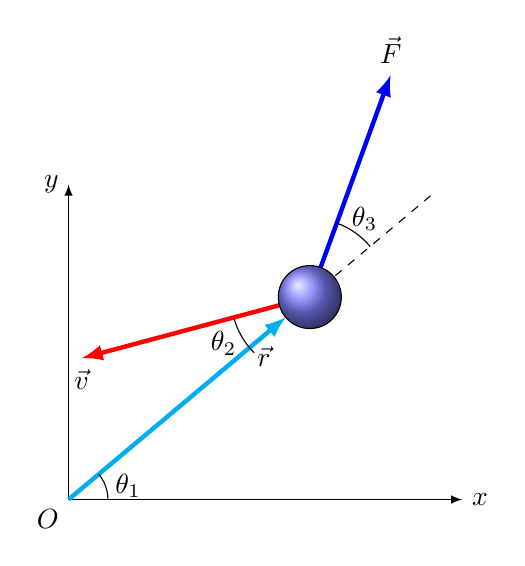
\begin{tikzpicture}
		\pgfmathsetmacro{\bang}{40}
		\pgfmathsetmacro{\bangtwo}{30}
		\pgfmathsetmacro{\bangthree}{30}
		\pgfmathsetmacro{\d}{4}
		\coordinate (P) at (\bang:\d);
		\coordinate (O) at (0,0);
		\pgfmathsetmacro{\Rb}{0.4}
		\node[below left] at (O) {$O$};
		\draw[-latex] (0,0) -- +(0,4) node[left] {$y$};
		\draw[-latex] (0,0) -- +(5,0) node[right] {$x$};
		\draw[ultra thick, cyan, -latex] (O) -- +(\bang:{\d-\Rb}) node[pos=0.9, below, text=black] {$\vec r$};
		\draw (O) +(0:0.5) arc(0:\bang:0.5) node[pos=0.5, right] {$\theta_1$};
		\draw (P) +({225-\bangtwo}:1) arc ({225-\bangtwo}:225:1) node[left, pos=0.7] {$\theta_2$};
		\draw[ultra thick, red, -latex] (P) -- +({225-\bangtwo}:3) node[below, text=black] {$\vec v$};
		\draw[dashed] (P) -- +(\bang:2);
		\draw[ultra thick, blue, -latex] (P) -- +({\bang + \bangthree}:3) node[above, text=black] {$\vec F$};
		\draw (P) +(\bang:1) arc (\bang:{\bang + \bangthree}:1) node[pos=0.2, text=black, above] {$\theta_3$};
		\draw[ball color= blue!50] (P) circle (\Rb);
	\end{tikzpicture}
	\captionof{figure}{Problem~\ref{prb:ang_mom_and_torque}}
	\label{ang_mom_and_torque}
	}%
	At the instant of Fig.~\ref{ang_mom_and_torque}, a $2.0$~kg particle $P$ has a position vector of magnitude $3.0$~m and angle $\theta_1 = \ang{45}$ and a velocity vector of magnitude $4.0$~m/s and angle $\theta_2 = \ang{30}$. Force $\vec F$ of magnitude $2.0$~N and angle $\theta_3 = \ang{30}$, acts on $P$. All three vectors lie in the $xy$ plane. About the origin, what are the 
	\begin{enumerate*}[label=(\alph*)]
		\item magnitude and
		\item direction of the angular momentum of $P$ and the
		\item magnitude and
		\item direction of the torque acting on $P$?
	\end{enumerate*}
\end{problem}

%=========================================================
\begin{problem}\correct{6.5cm}[4]%
	At time $t$, the vector $\vec r = 4.0t^2 \vec i - (2.0 t + 6.0t^2 ) \vec j$ gives the position of a $3.0$~kg particle relative to the origin of an $xy$ coordinate system ($\vec r$ is in meters and $t$ is in seconds). 
	\begin{enumerate*}[label=(\alph*)]
		\item Find an expression for the torque acting on the particle relative to the origin. 
		\item Is the magnitude of the particle’s angular momentum relative to the origin increasing, decreasing, or unchanging?
	\end{enumerate*}
	\begin{solution}
		\begin{enumerate*}[label=(\alph*)]
			\item $48t$~\si{\newton\meter}; 
			\item increasingю
		\end{enumerate*}
	\end{solution}
\end{problem}

%=========================================================
\begin{problem}\label{prb:ball_hit_dumbell}
	A ball of mass $m$ moving with velocity $v_0$ experiences a head-on elastic collision with one of the spheres of a stationary rigid dumbbell as whown in Fig.~\ref{ball_hit_dumbell}. The mass of each sphere equals $\nfrac{m}{2}$, and the distance between them is $l$. Disregarding the size of the spheres, find the proper angular momentum of the dumbbell after the collision, i.e. the angular momentum in the reference frame moving translationally and fixed to the dumbbell's centre of mass.
	\begin{solution}
		$L = \frac13 mv_0l$.
	\end{solution}
\end{problem}

%=========================================================
\begin{figure}[h!]\centering
	%---------------------------------------------------------
	\begin{minipage}[t]{0.45\linewidth}\centering
		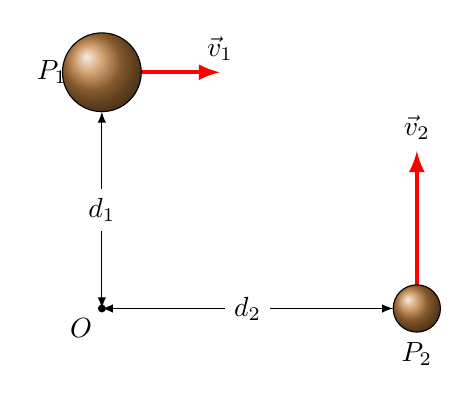
\begin{tikzpicture}
			\pgfmathsetmacro{\do}{3}
			\pgfmathsetmacro{\dt}{4}
			\pgfmathsetmacro{\Ro}{0.5}
			\pgfmathsetmacro{\Rt}{0.3}
			\coordinate (P1) at (0,\do);
			\coordinate (P2) at (\dt,0);
			\fill (0,0) node[below left] {$O$} circle (0.05);
			\draw[ultra thick, red, -latex] (P1) -- +(1.5,0) node[above, text = black] {$\vec v_1$}; 
			\draw[ultra thick, red, -latex] (P2) -- +(0,2) node[above, text = black] {$\vec v_2$}; 
			\draw[latex-latex] (0,0) -- node[fill=white] {$d_1$} ([yshift=-\Ro cm]P1);
			\draw[latex-latex] (0,0) -- node[fill=white] {$d_2$} ([xshift=-\Rt cm]P2);
			\draw[ball color = brown] (P1) node[left = {\Ro +0.3cm}] {$P_1$} circle (\Ro);
			\draw[ball color = brown] (P2) node[below = {\Rt + 0.3cm}] {$P_2$} circle (\Rt);
		\end{tikzpicture}
		\caption{Problem~\ref{prb:ang_mom_two_part}}
		\label{ang_mom_two_part}
	\end{minipage}
	%---------------------------------------------------------
	\begin{minipage}[t]{0.45\linewidth}\centering
		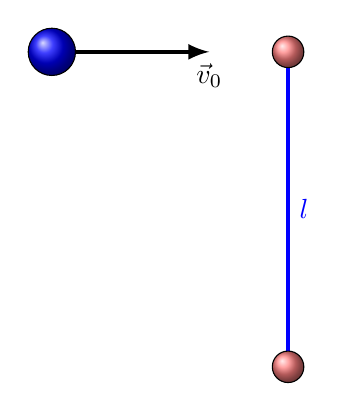
\begin{tikzpicture}
		\draw[blue, ultra thick] (2,2) -- node [right] {$l$}(2,-2);
		\draw[ball color=red!50] (2,2) circle (0.2);
		\draw[ball color=red!50] (2,-2) circle (0.2);
		\draw [ultra thick, -latex] (-1,2) -- +(2,0) node[below] {$\vec v_0$};
		\draw[ball color=blue] (-1,2) circle (0.3);		
		\end{tikzpicture}
		\caption{Problem~\ref{prb:ball_hit_dumbell}}
		\label{ball_hit_dumbell}
	\end{minipage}
	%---------------------------------------------------------
\end{figure}
%=========================================================
\Closesolutionfile{answer}

